\section{Introduction}
Acoustic scattering by elastic objects is a continuing area of study. Most phenomena in the scattering process can be adequately described by linear elasticity theory, and by further restricting the analysis to homogeneous, isotropic bodies of simple geometries, the mathematical formalism becomes simple enough to be handled by conventional analytic methods. 

The problems fall into mainly three categories: scattering of acoustic waves from elastic objects, scattering of elastic waves from fluid-filled cavities and solid inclusions, and inverse scattering, i.e., obtaining properties of a scattering object from the remotely sensed field. In the first category, the classical problems include scattering by spheres and infinite cylinders: fluid spheres~\cite{Anderson1950ssf}, solid spheres and cylinders~\cite{Faran1951ssb, Anderson1955soa, Hickling1962aoe, Doolittle1968ssb, Flax1978toe, Gaunaurd1983rao}, and spherical and cylindrical shells with various combinations of material properties~\cite{Hickling1964aoe, Doolittle1966ssb, Gaunaurd1987lac, Gaunaurd1991ssb, Kaduchak1998rbm, Chang1994voa, Chang1994soa, Fender1972sfa}. 
Much of the work in this field up to around 1980, is summarized in Flax et al.~\cite{Flax1981pa}.

The surrounding medium is usually considered to be a lossless fluid, but viscous fluids~\cite{Lin1983asb} and viscoelastic media and materials~\cite{Hasheminejad2005asf} are also considered. 

The acoustic illumination is often taken to be a plane wave which is relevant for far-field sources, otherwise point sources are applied in the near-field. For the infinite cylinder, the incident field is in most cases applied normal to the cylinder, but obliquely incident fields are also considered~\cite{Bao1990ras, Daneshjou2017aes}. More recently, the problem of scattering of beams has received much attention~\cite{Marston2007abs, Gong2016aso}. 

Solutions to some non-symmetric problems are also given; e.g. partially fluid filled spheres~\cite{Fawcett2001sfa}, spheres with eccentric cavities~\cite{Hasheminejad2005asf}, and open spheres with internal point sources~\cite{Elias1991sba}.

The studies mentioned above consider a single object in the free field. It is also of interest to study interactions between objects, and between an object and a boundary. The problem of multiple scattering is studied in e.g.~\cite{Gabrielli2001asb} for two elastic spheres, and in~\cite{Wu2006mso} for many fluid spheres, while the scattering by objects close to boundaries, and by  partially buried objects is addressed in~\cite{Zampolli2009bpf}.


%3) Other equations: 


Applications of the theory are numerous, and include scattering from marine life~\cite{Stanton1998dbs, Stanton2000asb, Anderson1950ssf}, various aspects of sonar, nondestructive testing, seismology, detection of buried objects~\cite{Sessarego1998sba}, medical imaging~\cite{Wells2006ui}, determination of material properties by inverse scattering~\cite{Ayres1987ias}, and acoustic cloaking. Acoustic cloaking, i.e., making an object acoustically 'invisible', requires acoustic metamaterials and is difficult to realize in practice, but reducing the backscattering strength of an object is an important issue, and can be realized either passively by coating or actively as suggested in e.g. \cite{Avital2015ssa}. 
A recent area of research is noise control in aerospace- and automotive engineering, where sound transmission through cylindrical shells constructed from new composite materials \cite{Talebitooti2016att} and functionally graded materials \cite{Daneshjou2017aes} are studied in order to reduce noise level inside the cabin. The latter problem requires a full 3D solution. %Full 3D, 

%{\em Method}
%Historically, the problem has been attacked in three steps: First, classical scattering %theory was used to solve the simple shapes. Second, RST analysis, and third, physical %interpretations of target resonances in terms of surface waves. 

The method referred to as classical scattering theory starts with the linearized elasto-dynamic equation of motion (also called Naviers equation). For the intended applications, nonlinear effects are negligible, which justifies the use of the linear approximation. For a certain class of coordinate systems, the field can be expressed in terms of three scalar potentials, which satisfy scalar Helmholtz equations, and admit solutions in the form of infinite series, termed normal modes or partial waves. The formal series expansions contain all the physical features of the solution, i.e., the reflected, transmitted and circumferential (or creeping) waves. The most general problems on finite scatterers in free space are scattering by the spherical shells which requires all three potentials and give solutions in terms of double sums. However, assuming axisymmetric illumination there is no loss of generality in aligning the coordinate axis of the sphere with the axis of the incident field, resulting in an axisymmetric problem. This results in a single infinite series which is much more computational efficient than the general case. This is the approach taken here.
 
%Truncation: 
As the solution is in the form of an infinite series, it needs to be truncated at some point. The summation is terminated when the relative magnitude of the last term is less than some prescribed tolerance, such that no computational parameters are introduced if this tolerance is chosen to be the precision used in the calculations (typically double precision). It is shown, by using symbolic precision in MATLAB, that the computational errors in the implementation are due to round-off errors. This is a natural definition of a computational exact solution.

The work reviewed above solves a host of different problems, and several reference solutions are available, with complexity up to three layers. What the present work provides is the explicit solution for a fully general multilayered sphere, and with corresponding analysis of the computational residual errors. This allows easy design and modeling of reference solutions for the purpose of validating numerical methods.
More specific, the model solves the problem of scattering by an incident plane wave, or wave from a point source, by spherical objects consisting of an arbitrary number of layers. Any combinations of fluid and solid layers can be handled, and the special cases of replacing the Neumann-to-Neumann condition by a single Neumann condition is also included.

%More precisely, we consider the problem of scattering by an incident plane wave, or wave from a point source, by spherical objects consisting of an arbitrary number of layers. The method handles any combination of fluid and solid layers, and the special cases of replacing the Neumann-to-Neumann condition by a single Neumann condition is also included.

%A set of benchmark problems is also suggested, consisting of three spherical shells of different diameter, which can be combined into a (symmetric) multilayered object. Solutions are provided to ...

   

An early work on scattering from multilayered spheres and infinite cylinders is Jenserud and Tollefsen~\cite{Jenserud1990ars}. The method employed here is referred to as the global matrix method~\cite{Schmidt1985afw} and is a systematic way of assembling local solutions for the individual layers into a global matrix for the total problem. 
The present work uses the same approach and builds mainly upon the work of Chang and Demkowicz~\cite{Chang1994voa}, which is generalized to multilayered spherical objects.

\begin{figure}
	\centering
	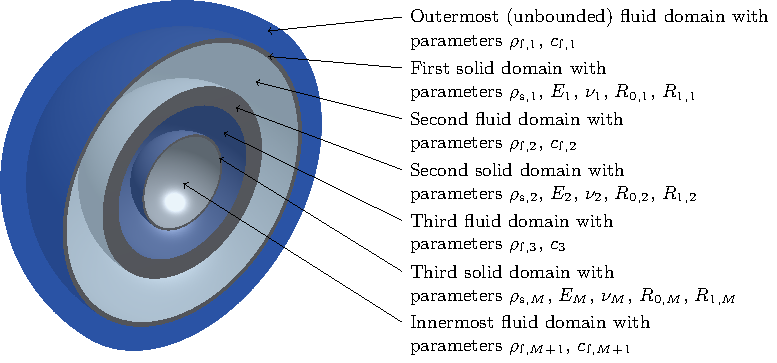
\includegraphics{../../LaTeX/createFigures/TikzFigures/article_e3Dss_PhD/parameters_distribution}
%	\includegraphics[scale=1]{\graphicsFolder/Figure1}
	\caption{A model with $M=3$ steel shells with different thicknesses (clip view), illustrating the distribution of the physical parameters over the different domains.}
	\label{Fig1:illustration}
\end{figure}

%Chang and Demkowicz solved the scattering problem on a spherical shell with vacuum fill in \cite{Chang1994voa2} (with additional vibration analysis in \cite{Chang1994voa1}). Goodman solved the problem for identical fluid inside and outside a single shell in~\cite{Goodman1962rat}, and Fender generalized this solution to different fluids inside and outside a single shell in~\cite{Fender1972sfa}. We shall build upon the work done in \cite{Chang1994voa2} and \cite{Fender1972sfa}, to generalize this even further to $M$ layers of shells (see \Cref{Fig1:illustration}). Moreover, we shall extend the solution to include scattering on solid spheres, rigid scattering and scattering on shells with vacuum fill.

